\documentclass[ignorenonframetext,xcolor=x11names]{beamer}

\input{../common.preamble.beamer.tex}

\title{Business 4720 - Class 22}

\subtitle{Reinforcement Learning -- Function Approximation}

\begin{document}

\begin{frame}{}
  \titlepage
  \footnotesize
  \input{../license.tex}
\end{frame}

\section{Introduction}

\begin{frame}{This Class}

\begin{block}{What You Will Learn:}
\begin{itemize}
  \item Reinforcement Learning
  \begin{itemize}
     \item Action-value approximation
     \item Policy approximation
  \end{itemize}
\end{itemize}
\end{block}
\end{frame}

\begin{frame}{Based On}
\begin{block}{}
Richard S. Sutton and Andrew G. Barto (2018) \emph{Reinforcement Learning -- An Introduction}. 2nd edition, The MIT Press, Cambridge, MA. (SB) \\
\vspace{0.5\baselineskip}
\url{http://incompleteideas.net/book/the-book.html} \\
\vspace{0.5\baselineskip}
Chapters 9--13
\end{block}

\begin{block}{}
Sudharsan Ravichandiran (2020) \emph{Deep Reinforcement Learning with Python}. 2nd edition. Packt Publishing, Birmingham, UK. \\
\vspace{0.5\baselineskip}
Chapters 9--11
\end{block}

\end{frame}

\begin{frame}{Resources}
Implementations are available on the following GitHub repo:

\url{https://github.com/jevermann/busi4720-rl} \\


The project can be cloned from this URL:

\url{https://github.com/jevermann/busi4720-rl.git}
\end{frame}


\begin{frame}{Function Approximation}
\begin{block}{Previously}
\begin{itemize}
\item Tabular methods only suitable for small state space and discrete actions
\end{itemize}
\end{block}

\begin{block}{Now}
\begin{itemize}
\item Approximate the state-value function $v$ by parameterized function $\hat{v}$:\\
\begin{center}
$\hat{v}(s) = \hat{v}(s, \theta) \approx v_{\pi}(s)$ \end{center}
\item Approximate the action-value function $q$ by a parameterized function $\hat{q}$: \\ \vspace{.25\baselineskip}
\begin{center}
$\hat{q}(s, a) = \hat{q}(s, a, \theta) \approx q_{\pi}(s, a)$
\end{center}
\item Approximate policy $\pi$ by a parameterized function $\hat{\pi}$: \\ \vspace{.25\baselineskip}
\begin{center}
$\hat{\pi}(a | s) = \hat{\pi}(a | s, \theta) \approx \pi(a | s)$
\end{center}
\end{itemize}
\end{block}
\end{frame}

\begin{frame}{Function Approximation}
\begin{block}{Advantages}
\begin{itemize}
\item Continuous states and/or actions
\item Tractable problems despite large state space
\item Flexible functions (linear, trees, neural networks)
\item Generalization to related states
\begin{itemize}
   \item Changing $\theta$ changes the values of multiple states
\end{itemize}
\item Applicable to partially observable problems
\begin{itemize}
   \item State function may not depend on complete state information
\end{itemize}
\end{itemize}
\end{block}
\end{frame}

\begin{frame}{Stochastic Gradient Methods}
Assume a MSE value error:
\begin{align*}
\bar{VE} = \sum_{s \in \mathcal{S}} \mu(s) \left[ q_\pi(s, a) - \hat{q}(s, a, \theta) \right]^2
\end{align*}
Follow the steepest slope (''gradient''; vector of partial derivatives) of the function to update parameters:
\begin{align*}
\theta_{t+1} &= \theta_t - \frac{1}{2} \alpha \nabla \left[ q_\pi(S_t, A_t) - \hat{q}(S_t, A_t,  \theta_t)\right]^2 \\
 &= \theta_t + \alpha \left[ q_\pi(S_t, A_t) - \hat{q}(S_t, A_t, \theta_t)\right] \nabla \hat{q}(S_t, A_t, \theta_t)
\end{align*}
True value $q_\pi(S_t, A_t)$ generally unknown; use an unbiased estimate $U_t = R_t + \gamma \hat{q}(S_{t+1}, A_{t+1}, \theta)$ instead:
\begin{align*}
\theta_{t+1} &= \theta_t + \alpha \left[ U_t - \hat{q}(S_t, A_t, \theta_t)\right] \nabla \hat{q}(S_t, A_t, \theta_t)
\end{align*}
\vspace{-\baselineskip}
\begin{block}{}
\textbf{Replace update to $Q$ with update to $\theta$}
\end{block}
\end{frame}

\begin{frame}{Example -- Semi-gradient SARSA}
\begin{block}{}
\begin{align*}
& \text{Initialize}\; \theta \in \mathbbm{R}^d \; \text{arbitrarily} \\
& \text{Loop for each episode:} \\
& \quad \text{Initialize}\; S_0 \\
& \quad \text{Choose}\; A \; \text{as a function of}\; \hat{q}(S_0, ., \theta) \; \text{e.g., $\epsilon$-greedy} \\ 
& \quad \text{Loop for each step of episode:} \\
& \quad \quad \text{Take action}\; A, \; \text{observe} \; R, S' \\
& \quad \quad \text{Choose}\; A' \; \text{as a function of}\; \hat{q}(S', ., \theta) \; \text{e.g., $\epsilon$-greedy} \\ 
& \quad \quad \theta \leftarrow \theta + \alpha [R + \gamma \hat{q}(S', A', \theta) - \hat{q}(S, A, \theta)] \nabla \hat{q}(S, A, \theta) \\
& \quad \quad S \leftarrow S'; A \leftarrow A' \\
& \quad \text{until S is terminal}
\end{align*}
\vspace{-\baselineskip}
\end{block}
\end{frame}

%\begin{frame}{Off-Policy TD Learning -- Q-Learning}
%\begin{block}{}
%\begin{align*}
%& \text{Initialize}\; Q(s, a) \; \text{for all} \; s \in \mathcal{S}^+ \; \text{, arbitrarily} \\
%& \text{Loop for each episode:} \\
%& \quad \text{Initialize}\; S \\
%& \quad \text{Loop for each step of episode:} \\
%& \quad \quad \text{Choose} \, A \, \text{from}\, S \, \text{using policy derived from} \, Q \\
%& \quad \quad \text{Take action}\, A, \, \text{observe} \, R, S' \\
%& \quad \quad Q(S, A) \leftarrow Q(S, A) + \alpha \left[ R + \gamma \operatorname*{max}_a Q(S', A') - Q(S, A) \right] \\
%& \quad \quad S \leftarrow S' \\
%& \quad \text{until}\, S\, \text{is terminal}
%\end{align*}
%\end{block}
%\end{frame}


\begin{frame}{''The Deadly Triad''}
\textbf{Instability} and \textbf{Divergence} arise when combining all three elements:
\begin{itemize}
\item \textbf{Function approximation}: Generalizing from a state space using linear functions or neural networks
\item \textbf{Bootstrapping}: Targets include existing estimates (e.g. SARSA) rather than actual rewards only (e.g. MC methods)
\item \textbf{Off-policy training}: Training on a distribution of transitions other than that produced by the target policy
\end{itemize}
\end{frame}

\begin{frame}{DQN -- Double Q Network}
\begin{block}{Experience Replay}
\begin{itemize}
  \item Store sequences $S, A, R, S', A'$ in \emph{replay buffer}
  \item FIFO queue of limited size
  \item Sample from replay buffer for each batch
  \item Removes/limits correlation of states within batches
  \item Smoothes data distribution changes
\end{itemize}
\end{block}
\begin{block}{Target Network}
\begin{itemize}
   \item Maintain stable targets during updates
   \item Periodic update from ''main'' network
\end{itemize}
\end{block}
\end{frame}

\begin{frame}{DQN -- Algorithm}
\footnotesize
\begin{block}{}
\vspace{-\baselineskip}
\begin{align*}
& \text{Init replay buffer}\;D \leftarrow \emptyset \\
& \text{Init main action-value function approximation}\;\hat{q}_M\;\text{with random parameters}\;\theta_M \\
& \text{Init target action-value function approximation}\;\hat{q}_T\;\text{with paramaters}\;\theta_T=\theta_M \\
& \text{Loop for each episode:}\\
& \quad \text{Initialize}\;S \\
& \quad \text{For each step of the episode:} \\
& \quad \quad \text{Select action}\; A \; \text{using an} \; \text{$\epsilon$-greedy policy based on}\; \hat{q_M}\\
& \quad \quad \text{Take action} \; A \; \text{and observe}\;R, S_{t+1} \\
& \quad \quad \text{Store transition} \; (S_t , A_t , R_t , S_{t+1} ) \; \text{in} \; D \\
& \quad \quad \text{Sample minibatch} \; (S_j , A_j , R_j , S_{j+1} ) \; \text{from} \; D \\
& \quad \quad \text{Target}\;y_j \leftarrow \begin{cases} r_j & \qquad \quad \text{if $S_{j+1}$ is terminal} \\
r_j + \gamma \max_{A'} \hat{q}_T(S_{j+1}, A'; \theta_T) & \qquad \quad \text{otherwise}\end{cases} \\
& \quad \quad \theta_M \leftarrow \theta_M + \alpha [y_j - \hat{q}_M (S_j, A_j, \theta_M)] \nabla \hat{q}_M(S_j, A_j, \theta_M) \hspace{1in} \\
%& \quad \quad \text{Perform a gradient descent step on loss function}\;L=\left[y_j-\hat{q}_M(S_j,a_j;\theta_M)\right]^2 \\
& \quad \text{Every $C$ steps, update}\; \hat{q}_T \leftarrow \hat{q}_M\;\text{by setting}\; \theta_T \leftarrow \theta_M
\end{align*}
\vspace{-\baselineskip}
\end{block}
\end{frame}

\begin{frame}{DQN -- Algorithm}
\begin{itemize}
   \item In practice, $S$ is a function $\phi(X)$ of inputs $X$ through feature-extraction and pre-processing
   \item In practice, the update $y_j - Q(S_j, a_j, \theta)$ is clipped to $[-1, 1]$
   \end{itemize}
\end{frame}

\begin{frame}{DQN Example -- Cart Pole}
\centering
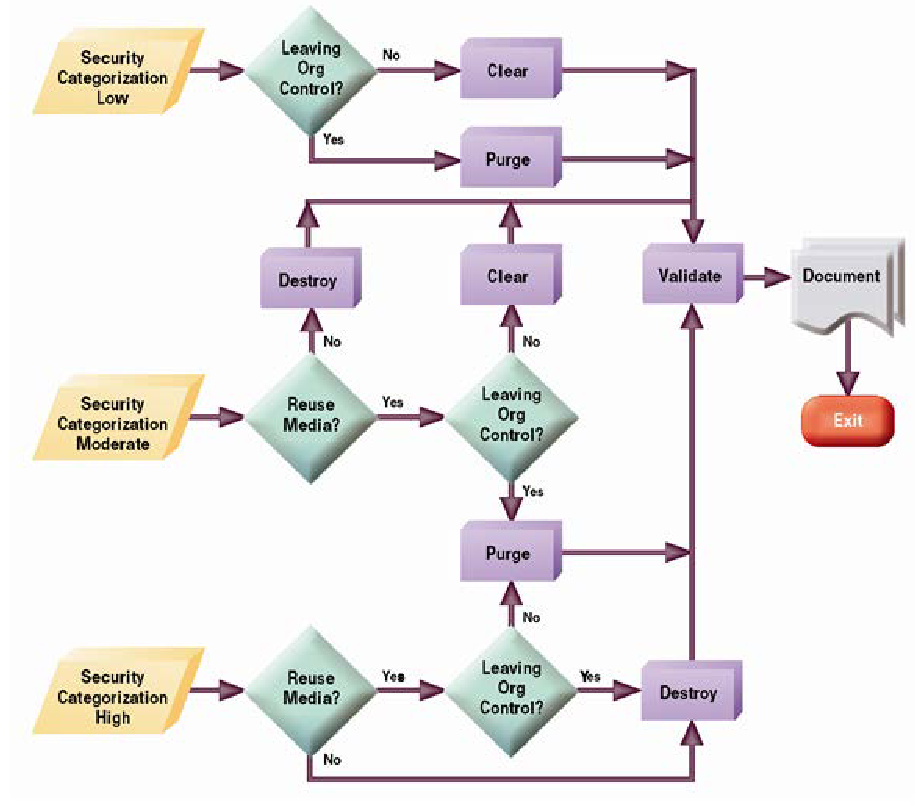
\includegraphics[height=2.5in]{screen1.png}
\end{frame}

\begin{frame}{DQN Example -- Cart Pole}
\small
\textbf{Action Space}:
\begin{center}
\begin{tabular}{c|l} \hline
0 & Push cart to the left \\
1 & Push cart to the right \\ \hline
\end{tabular}
\end{center}


\textbf{State/feature space}:
\begin{center}
\begin{tabular}{c|l|l|l} \hline
\emph{Num} & \emph{Observation} & \emph{Min} & \emph{Max} \\ \hline
0 & Cart position & -4.8 & 4.8 \\
1 & Cart velocity & -Inf & Inf \\
2 & Pole angle & -24 deg & 24 deg \\
3 & Pole angular velocity & -Inf & Inf \\ \hline
\end{tabular}
\end{center}

\textbf{Rewards} are +1 for every step taken \\

\textbf{Termination} occurs either:
\begin{itemize}
\item Pole angle is greater than $\pm 12$ deg
\item Cart position is greater than $\pm 2.4$
\item Episode length is grater than 200
\end{itemize}
\end{frame}


\begin{frame}[fragile]{DQN in Python}
Use the ''CartPole'' environment from \url{https://gymnasium.farama.org/}:
\begin{pythoncode}
import math
import random
import keras
from keras import layers
import gymnasium as gym
import tensorflow as tf
import numpy as np
import pygame

env = gym.make("CartPole-v1", render_mode="human")

Actions = range(0, env.action_space.n)
Ssize = env.observation_space.shape[0]
\end{pythoncode}
\end{frame}


\begin{frame}[fragile]{DQN in Python \small [cont'd]}
Neural network and RL hyperparameters:
\begin{pythoncode}
# Neural net parameters
batch_size = 8
dropout = 0.25
activation = 'relu'

epsilon = 0.8 # initial epsilon
gamma = 0.9 # discount factor
neps = 1000 # dicreasing epsilon factor
C = 50*batch_size # When to update weights

# Replay buffer D
D = collections.deque(maxlen=5000)
\end{pythoncode}
\end{frame}

\begin{frame}[fragile]{DQN in Python \small [cont'd]}
Define the neural networks:
\begin{pythoncode}
# Main network, used to select actions
Q = keras.Sequential([
    layers.InputLayer(input_shape=(Ssize+1),
                      batch_size=batch_size,
                      dtype=tf.float32),
    layers.Dense(Ssize*4, activation=activation),
    layers.Dropout(rate=dropout),
    layers.Dense(Ssize*2, activation=activation),
    layers.Dropout(rate=dropout),
    layers.Dense(1, activation='linear')
])
Q.compile(loss='huber', optimizer='adam')

# Target network, used to compute targets
Qhat = keras.models.clone_model(Q)
Qhat.compile(loss='huber', optimizer='adam')
Qhat.set_weights(Q.get_weights())
\end{pythoncode}
\end{frame}

\begin{frame}[fragile]{DQN in Python \small [cont'd]}
Getting a $Q(s, a)$ value involves predicting from the neural net:
\begin{pythoncode}
def getQ(Q, s, a):
    return Q.predict(np.expand_dims(np.array( \
        s.tolist()+[a]), axis=0), verbose=0)[0][0]
\end{pythoncode}
Max/Argmax operator for $Q(s, a)$ using prediction from main or target network:
\begin{pythoncode}
def maxQ(Q, s, arg):
    maxq = -np.inf
    maxa = None
    for a in Actions:
        q = getQ(Q, s, a)
        if q > maxq:
            maxq = q
            maxa = a
    return maxa if arg else maxq
\end{pythoncode}
\end{frame}

\begin{frame}[fragile]{DQN in Python \small [cont'd]}
$\epsilon$-greedy policy $pi_\epsilon(s)$
\begin{pythoncode}
def pi(s, epsilon):
    if random.random() < epsilon:
        return random.choice(Actions)
    else:
        return maxQ(Q, s, True)
\end{pythoncode}
Update target for DQN:
\begin{pythoncode}
def target_DQN(Q, Qhat, a, r, sprime):
    return r + gamma * maxQ(Qhat, sprime, False)
\end{pythoncode}
Update target for DDQN:
\begin{pythoncode}
def target_DDQN(Q, Qhat, a, r, sprime):
    return r + gamma * getQ(Qhat, sprime, \ 
                               maxQ(Q, sprime, False))
\end{pythoncode}
\end{frame}

\begin{frame}[fragile]{DQN in Python \small [cont'd]}
Creating x and y data for training:
\begin{pythoncode}
def training_xy(batch, ddqn=False):
    x = np.zeros((batch_size, Ssize+1))
    y = np.zeros(batch_size)
    for i, (s, a, r, t, sprime) in enumerate(batch):
        x[i] = list(s) + [a]
        if t == 1:
            y[i] = r
        else:
            if ddqn:
                y[i]=target_DDQN(Q, Qhat, a, r, sprime)
            else:
                y[i]=target_DQN(Q, Qhat, a, r, sprime)
    return x, y
\end{pythoncode}
\end{frame}

\begin{frame}[fragile]{DQN in Python \small [cont'd]}
DQN/DDQN code:
\begin{pythoncode}
for t in range(max_steps):
    s = env.reset()[0]
    a = pi(s, epsilon*math.exp(-t/neps))
    sprime, r, terminal, _, _ = env.step(a)
    G += r
    D.append((s, a, r, int(terminal), sprime))
    s = sprime
    if t >= batch_size:
        batch = random.sample(D, batch_size)
        x, y = training_xy(batch, ddqn=True)
        loss = Q.train_on_batch(x=x, y=y)

    if t % C == 0:
        Qhat.set_weights(Q.get_weights())
\end{pythoncode}

Complete code at \url{https://evermann.ca/busi4720/DDQN_tuples.py}
\end{frame}

\begin{frame}{DQN Extensions}
\begin{block}{Prioritized Experience Replay (PEX)}
\begin{itemize}
   \item Important actions are sampled with higher probability
   \item Use absolute TD error as priorities
   \item Faster learning
\end{itemize}
\end{block}

\begin{block}{Double DQN}
\begin{itemize}
   \item Based on Double Q-Learning
   \item Uses target network $\hat{Q}$ as second $Q$ function
   \item Removes upwards bias from using \emph{max()} functions as estimator
\end{itemize}
\end{block}
\end{frame}

\begin{frame}{Advantage Function}
\begin{align*}
A(s, a) = Q(s, a) - V(s)
\end{align*}
\textbf{Advantage of action $a$ in state $s$ over the average action in state $s$} \\

Rewrite as:
\begin{align*}
Q(s, a) = V(s) + A(s, a)
\end{align*}
\end{frame}

\begin{frame}{Dueling DQN}
\begin{itemize}
   \item Neural network from features $x$ for value function $V(s)$ (''value stream'')
   \item Neural network from features $x$ for advantage function $A(s, a)$ (''advantage stream'')
   \item Typically, value stream and advantage stream follow one or more common layers
   \item Aggregate to compute $Q(s, a)$
\end{itemize}
\begin{align*}
Q(s, a, \theta, \alpha, \beta) = V(s, \theta, \beta) + \left( A(s, a, \theta, \alpha) - \frac{a}{|\mathcal{A}|} A(s, a', \theta, \alpha) \right)
\end{align*}
Where $\theta$ are shared neural-network parameters, $\beta$ are parameters only for the ''value-stream'' neural network, and $\alpha$ are parameters only for the ''advantage-stream'' neural network
\end{frame}

\begin{frame}{Policy Gradient Methods}
\begin{block}{Idea}
Learn a parameterized policy :
\begin{align*}
\pi(s, a) = \pi(s, a, \theta) = \Pr(A_t = a | S_t = s, \theta_t = \theta)
\end{align*}
Optimize:
\begin{align*}
J(\theta) = v_{\pi_\theta}(s_o)
\end{align*}
\end{block}
\end{frame}

\begin{frame}{Policy Gradient Methods}
\begin{block}{Advantages}
\begin{itemize}
   \item Simpler to approximate than action-value function
   \item Selection of actions with arbitrary probabilities
   \item Can better approach deterministic policy than $\epsilon$-greedy action selection over action values
   \item Suitable for large and continuous action spaces
\end{itemize}
\end{block}
\end{frame}

\begin{frame}{Policy Gradient Methods}
REINFORCE update:
\begin{align*}
\theta_{t+1} = \theta_t + \alpha G_t \frac{\nabla \pi(A_t | S_t, \theta)}{\pi(A_t | S_t, \theta_t)}
\end{align*}
\begin{itemize}
   \item Update proportional to return $G_t$
   \item Update inversely proportional to action probability $\pi$
\end{itemize}
\end{frame}

\begin{frame}{Policy Gradient Methods}
\begin{block}{REINFORCE: Monte-Carlo Control (episodic)}
\begin{align*}
& \text{Input: A differentiable policy}\;\pi(a | s, \theta);\;\text{step size}\; \alpha > 0 \\
& \text{Initialize policy parameters}\; \theta \in \mathbbm{R}^d\;\text{arbitrarily} \\
& \text{Loop forever (for each episode):} \\
& \quad \text{Generate an episode}\; S_0, A_0, R_1, \ldots S_{T-1}, A_{T-1}, R_T, \\
& \quad \text{Loop for each step of the episode}\;t=0, 1, \ldots, T-1:\\
& \quad \quad G \leftarrow \sum\nolimits_{k=t+1}^T \gamma^{k - t - 1}R_k \\
& \quad \quad \theta \leftarrow \theta + \alpha G \nabla \ln \pi(A_t | S_t, \theta)
\end{align*}
\end{block}
\end{frame}

\begin{frame}[fragile]{REINFORCE in Python}
Policy function/network for discrete actions:
\begin{pythoncode}
# Batch size of 1 as we update after every action
p_net = keras.Sequential([
    layers.InputLayer(batch_input_shape=(1, Ssize), 
        dtype=tf.float32),
    layers.Dense(Ssize*4, activation='relu'),
    layers.Dropout(rate=0.25),
    layers.Dense(Ssize*2, activation='relu'),
    layers.Dropout(rate=0.25),
    layers.Dense(len(Actions), activation='softmax')
])
\end{pythoncode}
Action selection using policy network probabilities:
\begin{pythoncode}
def select_action(state):
    probs = p_net(np.expand_dims(state, axis=0))[0].numpy()
    action = np.random.choice(Actions, size=1, p=probs)[0]
    return action
\end{pythoncode}
\end{frame}

\begin{frame}[fragile]{REINFORCE in Python \small [cont'd]}
Generate an episode:
\begin{pythoncode}
# Do this for each episode
for e in range(neps):
    # Initialize variables and lists
    T = 0
    rewards, states, actions = [], [], []
    # Reset environment
    s = env.reset()[0]
    terminal = False
    # Generate an episode and keep track
    # of states, actions, rewards
    while (T < max_steps) and not terminal:
        a = select_action(s)
        sprime, r, terminal, _, _ = env.step(a)
        states.append(s)
        actions.append(a)
        rewards.append(r)
        s = sprime
        T += 1

    print(f'Episode {e:5} goes to step {T:3}')
    # Compute discounted returns
    returns = discounted_returns(rewards, gamma)
\end{pythoncode}
\end{frame}

\begin{frame}[fragile]{REINFORCE in Python \small [cont'd]}
Learning from episode:
\begin{pythoncode}
    # Learn for each step of the episode
    for t in range(len(returns)):
        with tf.GradientTape() as tape:
            # Action probabilities
            pi = p_net(np.expand_dims(states[t], axis=0))
            # Action index
            action_idx = np.array(actions[t], dtype=np.int32)
            # Return
            G = np.array(returns[t])
            # Loss
            loss = - G * gamma**t * 
                tf.math.log(tf.reduce_sum(tf.math.multiply(pi, 
                    tf.one_hot(action_idx, env.action_space.n)), 
                        axis=1))

        # Calculate gradients and update parameters
        grads = tape.gradient(loss, p_net.trainable_variables)
        optimizer.apply_gradients(zip(grads, 
            p_net.trainable_variables))
\end{pythoncode}
\end{frame}


\begin{frame}{Policy Gradient Methods}
REINFORCE with a baseline $b(S_t)$:
\begin{align*}
\theta_{t+1} = \theta_t + \alpha(G_t - b(S_t)) \frac{\nabla \pi(A_t | S_t, \theta)}{\pi(A_t | S_t, \theta_t)}
\end{align*}
Choose $b(S_t) = \hat{v}(S_t)$ the state-value function:
\begin{align*}
\theta_{t+1} = \theta_t + \alpha(G_t - \hat{v}(S_t)) \frac{\nabla \pi(A_t | S_t, \theta)}{\pi(A_t | S_t, \theta_t)}
\end{align*}
\begin{itemize}
   \item Baseline leaves the expected value unchanged (unbiased)
   \item Can significantly reduce the variance
   \item Can improve speed of learning
\end{itemize} 
\end{frame}

\begin{frame}{Policy Gradient Methods}
\begin{block}{REINFORCE with Baseline (episodic)}
\vspace{-.5\baselineskip}
\begin{align*}
& \text{Input: A policy}\;\pi(a | s, \theta);\;\text{step size}\; \alpha_\theta > 0 \\
& \text{Input: A state-value function}\;\hat{v}(s, w);\;\text{step size}\; \alpha_w > 0 \\
& \text{Initialize parameters}\; \theta \in \mathbbm{R}^d,\; w \in \mathbbm{R}^d\;\text{arbitrarily} \\
& \text{Loop forever (for each episode):} \\
& \quad \text{Generate an episode}\; S_0, A_0, R_1, \ldots S_{T-1}, A_{T-1}, R_T, \\
& \quad \text{Loop for each step of the episode}\;t=0, 1, \ldots, T-1:\\
& \quad \quad G \leftarrow \sum\nolimits_{k=t+1}^T \gamma^{k - t - 1}R_k \\
& \quad \quad \delta \leftarrow G - \hat{v}(S_t, w) \\
& \quad \quad w \leftarrow w + \alpha_w \delta \nabla \hat{v}(S_t, w) \\
& \quad \quad \theta \leftarrow \theta + \alpha_\theta \gamma^t G \nabla \ln \pi(A_t | S_t, \theta)
\end{align*}
\vspace{-.5\baselineskip}
\end{block}
\end{frame}

\begin{frame}[fragile]{REINFORCE with Baseline in Python \small [cont'd]}
Learning from episode:
\begin{pythoncode}
for t in range(len(returns)):
    with tf.GradientTape() as p_tape:
        with tf.GradientTape() as v_tape:
            pi = policy_network(np.expand_dims(states[t], axis=0))
            action_idx = np.array(actions[t], dtype=np.int32)
            # Value function
            v = value_network(np.expand_dims(states[t], axis=0))
            # Return
            G = np.array(returns[t])
            delta = G - v
            # Losses for policy and value networks
            p_loss = -delta * gamma**t * tf.math.log(tf.reduce_sum(tf.math.multiply(pi, tf.one_hot(action_idx, env.action_space.n)), axis=1))
            v_loss = -delta * v

    # Calculate gradients and update parameters for policy network
    p_grads = p_tape.gradient(p_loss,p_net.trainable_variables)  
    p_optimizer.apply_gradients(zip(p_grads, 
        p_net.trainable_variables))
    # Calculate gradients and update parameters for value network
    v_grads = v_tape.gradient(v_loss,v_net.trainable_variables)
    v_optimizer.apply_gradients(zip(v_grads, 
        v_network.trainable_variables))
\end{pythoncode}
\end{frame}


\begin{frame}{Policy Gradient Methods}
\textbf{One-Step Actor-Critic}:
\begin{align*}
\theta_{t+1} &= \theta_t + \alpha (G_{t} - \hat{v}(S_t)) \frac{\nabla \pi(A_t | S_t, \theta)}{\pi(A_t | S_t, \theta_t)} \\
&= \theta_t + \alpha (R_{t+1} + \gamma \hat{v}(S_{t+1}, w) - \hat{v}(S_t, w)) \frac{\nabla \pi(A_t | S_t, \theta)}{\pi(A_t | S_t, \theta_t)} \\
&= \theta_t + \alpha \delta_t \frac{\nabla \pi(A_t | S_t, \theta)}{\pi(A_t | S_t, \theta_t)}
\end{align*}
\begin{itemize}
  \item Analogous to TD, SARSA and Q-Learning for tabular methods
  \item Improve on slow learning of MC methods
  \item Useful for non-episodic, continuous problems
\end{itemize}
\end{frame}

\begin{frame}{Policy Gradient Methods}
\small
\begin{block}{One-Step Actor-Critic}
\vspace{-.5\baselineskip}
\begin{align*}
& \text{Input: A policy}\;\pi(a | s, \theta);\;\text{step size}\; \alpha_\theta > 0 \\
& \text{Input: A state-value function}\;\hat{v}(s, w);\;\text{step size}\; \alpha_w > 0 \\
& \text{Initialize parameters}\; \theta \in \mathbbm{R}^d,\; w \in \mathbbm{R}^d\;\text{arbitrarily} \\
& \text{Loop forever (for each episode):} \\
& \quad \text{Initialize}\;S\;\text{(first state of episode)}; I \leftarrow 1 \\
& \quad \text{Loop while}\;S\;\text{not terminal (for each time step):} \\
& \quad \quad \text{Sample}\;A\;\text{from}\; \pi(.|S, \theta) \\
& \quad \quad \text{Take action}\;A,\;\text{observe}\;S', R \\
& \quad \quad \delta \leftarrow R + \gamma \hat{v}(S', w) - \hat{v}(S, w) \\
& \quad \quad w \leftarrow w + \alpha_w \delta \nabla \hat{v}(S_t, w) \\
& \quad \quad \theta \leftarrow \theta + \alpha_\theta G \nabla \ln \pi(A_t | S_t, \theta) \\
& \quad \quad S \leftarrow S'; I \leftarrow \gamma I
\end{align*}
\vspace{-\baselineskip}
\end{block}
\end{frame}

\begin{frame}{Reference Implementations}
\small
\begin{block}{Stable Baselines}
\begin{itemize}
   \item Reference Python implementation of RL algorithms
   \item Pre-trained agents (''Baselines Zoo'')
   \item Originally developed at OpenAI
   \item Pointers to additional learning materials
\end{itemize}
\vspace{.5\baselineskip}
\url{https://stable-baselines.readthedocs.io/en/master/}
\end{block}
\begin{block}{Gymnasium}
\begin{itemize}
   \item A standard programming interface (API) for RL environments
   \item Collection of reference environments
   \item Originally developed at OpenAI
\end{itemize}
\vspace{.5\baselineskip}
\url{https://gymnasium.farama.org/index.html}
\end{block}
\end{frame}

\begin{frame}{AlphaGo}
\footnotesize
\begin{columns}
\begin{column}{0.45\textwidth}
\begin{center}
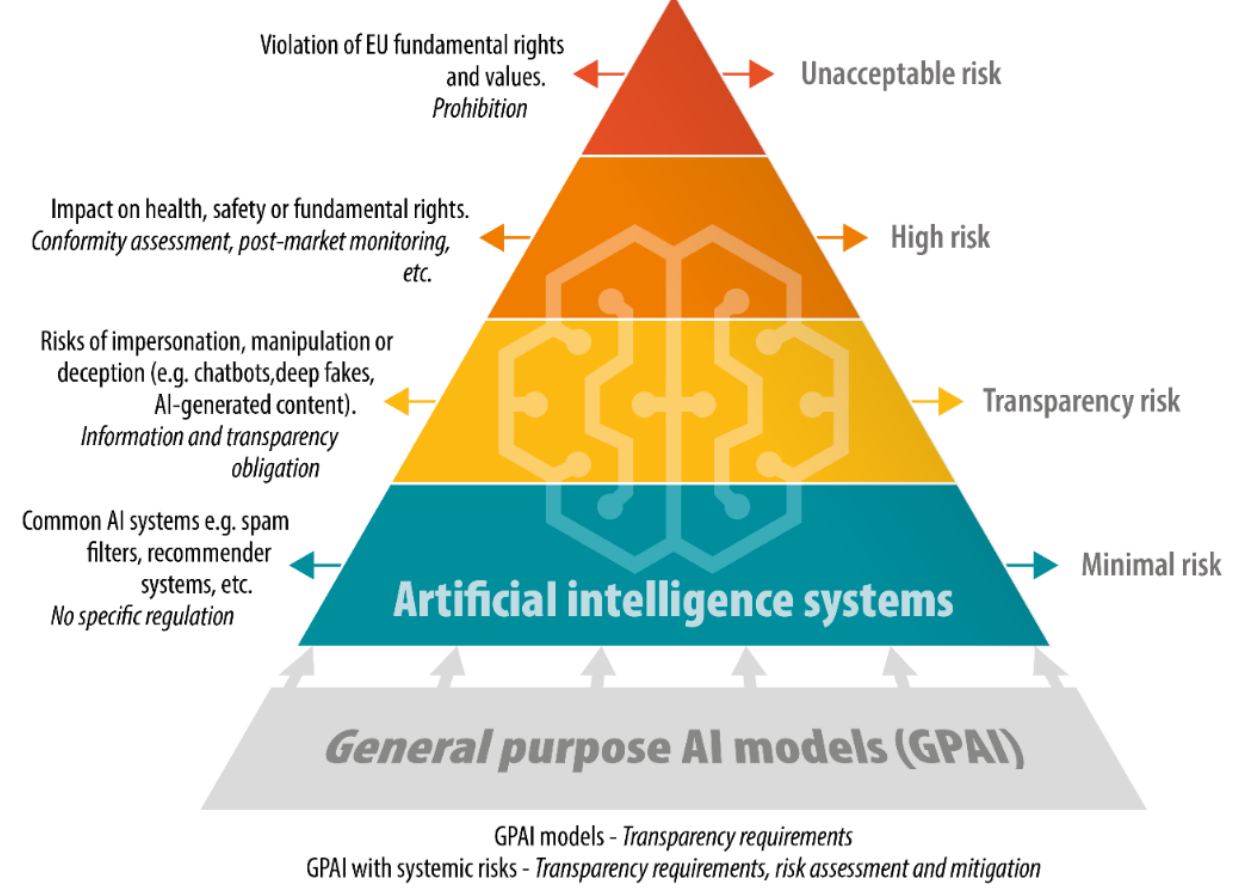
\includegraphics[height=2.5in]{screen2} \\
\tiny \url{https://www.alphagomovie.com} \footnotesize
\end{center}
\end{column}
\begin{column}{0.55\textwidth}
Google's DeepMind division became famous in 2017 when it trained a computer to beat the human world champion at the game of Go. An award-winning full-length documentary has been made about this achievement. \\
\vspace{\baselineskip}
\url{https://www.alphagomovie.com} \\
\url{https://www.youtube.com/watch?v=WXuK6gekU1Y} \\
\vspace{\baselineskip}
The introductory paper by David Silver and others in Nature should be easy to understand: ''Mastering the game of Go without human knowledge''. Nature. 550 (7676): 354--359\\ \url{https://www.nature.com/articles/nature24270}
\end{column}
\end{columns}
\end{frame}


\begin{frame}[allowframebreaks]{Additional Materials}
\footnotesize
\begin{block}{David Silver, UCL and Google DeepMind}
Dr. Silver (\url{https://www.davidsilver.uk/}) of University College London has an excellent introductory course on reinforcement learning with class materials (from 2015) and lectures in a YouTube playlist. Updated courses (2018, 2021) are available on the DeepMind YouTube channel. The 2021 course include topics on deep reinforcement learning. \\
\vspace{\baselineskip}
\url{https://www.davidsilver.uk/teaching/} \\
\vspace{.5\baselineskip}
\url{https://www.youtube.com/playlist?list=PLqYmG7hTraZDM-OYHWgPebj2MfCFzFObQ}. \\
\vspace{.5\baselineskip}
\url{https://www.youtube.com/@Google_DeepMind/playlists}.
\end{block}

\begin{block}{UC Berkeley}
UC Berkeley hosted a Deep RL Bootcamp in 2017 with slides and lecture videos available online. Additionally, UC Berkeley's course on Deep RL is available online, with lecture slides and videos of past years.
\vspace{\baselineskip}
\url{https://sites.google.com/view/deep-rl-bootcamp/lectures}
\vspace{\baselineskip}
\url{https://rail.eecs.berkeley.edu/deeprlcourse/}
\end{block}

\begin{block}{Denny Britz}
Formerly at the Google AI team, Denny Britz applied RL algorithms to financial markets and trading. He has a interesting blog, and a GitHub repository with resources and algorithm implementations of popular RL algorithms. \\
\vspace{\baselineskip}
\url{https://dennybritz.com/}
\vspace{\baselineskip}
\url{https://github.com/dennybritz/reinforcement-learning}
\end{block}

\begin{block}{Massimiliano Patacchiola, Cambridge University} 
Dr. Patacchiola is a postdoc at Cambridge University. He has written a series of excellent blog posts on reinforcement based on the book ''Artificial Intelligence -- A Modern Approach'' by Russell and Norvig. There are lots of illustrations and pointers to implementation and code in multiple languages. \\
\vspace{\baselineskip}
\url{https://github.com/mpatacchiola/dissecting-reinforcement-learning}
\end{block}

\begin{block}{Pascal Poupart, University of Waterloo}
Dr. Poupart has made available videos and all course materials for all lectures for a course on reinforcement learning at UWaterloo. \\
\vspace{.5\baselineskip}
\url{https://www.youtube.com/playlist?list=PLdAoL1zKcqTXFJniO3Tqqn6xMBBL07EDc} \\
\vspace{.5\baselineskip}
\url{https://cs.uwaterloo.ca/~ppoupart/teaching/cs885-spring18/schedule.html}
\end{block}

\begin{block}{Andrew Ng, Stanford University}
Dr. Ng (\url{https://www.andrewng.org/}) has taught an introductory class on reinforcement learning, as part of a broader course on machine learning. \\
\vspace{\baselineskip}
\url{https://www.youtube.com/watch?v=RtxI449ZjSc} \\
\vspace{.5\baselineskip}
\url{https://www.youtube.com/playlist?list=PLA89DCFA6ADACE599}
\end{block}

\begin{block}{Andrei Karpathy, OpenAI, formerly Tesla}
Andrei Karpathy (\url{https://karpathy.ai/} was a founding member of OpenAI (makers of ChatGPT and Dall-E) and later became the Tesla lead for their Autopilot program. An early blog post by Andrei Karpathy on RL is at the introductory level. \\
\vspace{.5\baselineskip}
\url{https://karpathy.github.io/2016/05/31/rl/}
\end{block}

\begin{block}{Lilian Weng, OpenAI}
Dr. Weng (\url{https://lilianweng.github.io/}) is a lead researchers at OpenAI (makers of ChatGPT and Dall-E). She has written an early blog post on RL and another one on policy gradient algorithms. \\
\vspace{.5\baselineskip}
\url{https://lilianweng.github.io/posts/2018-02-19-rl-overview/}\\
\vspace{.5\baselineskip}
\url{https://lilianweng.github.io/posts/2018-04-08-policy-gradient/}
\end{block}

\begin{block}{OpenAI}
OpenAI (\url{https://openai.com}; makers of ChatGPT and Dall-E) post regularly on their blog, on all things deep learning and also reinforcement learning. The blog posts are easy introduction to a variety of analytics topics. \\
\vspace{.5\baselineskip}
\url{https://openai.com/blog/openai-baselines-ppo/} \\
\vspace{.5\baselineskip}
\url{https://openai.com/blog/evolved-policy-gradients/} \\
\vspace{.5\baselineskip}
\url{https://openai.com/blog/evolution-strategies/}
\end{block}

\end{frame}






\end{document}



